







\chapter{}


\section{Punctuated equilibria — Gould may have got it right,  but maybe  the Vajrayana schools beat him to it}


Change is a consistent fact of life.

But change does not occur gradually or constantly; it churns at times, more vivaciously than others.

At these times — relative bursts of undetermined chaotic manifestation — the future gets decided by a long series of happenstances, each of which might seem inconsequential at the time. Together, they draw out an arc through tremendous divergences of possibilities: both into the future worlds of better circumstances, but also, and more largely, down into less favorable ones.

Periods of relative dynamic stasis are interspersed by upheavals of varying magnitude with unpredictable consequences. Like earthquakes, they release built-up tension that gets triggered by some alignment of forces that were ready to give way \cite{bak1991self}.

I feel it is this property of punctuated unfolding through time that Padmasambhava may have been onto when he wrote the Bardo Thodol. Bardos are transitory phases through which passage can lead to a number of varying eventualities. The idea is something like: the sum total of what “you” (and perhaps those with you) have “done” — your karma — will, in theory, influence your passage through the transition.

There are also bardos of becoming in evolutionary processes. At certain (relatively short) periods in history, there has been great flux, more substantial than the background average.

\section{Brief overview of the main Buddhist schools}

For reference, Vajrayana translates crudely to “the way of the lightning bolt.” Of Theravada (Hinayana — lesser vehicle), Mahayana (greater vehicle), and Vajrayana, Vajrayana Buddhist practices supposedly offer the fastest route to enlightenment. Theravada (Hinayana) is the orthodox school, which still follows the Pali Canon. It is still practiced in Sri Lanka, and much of Southeast Asia, especially Myanmar, Thailand, Laos, and Cambodia. Critics of Theravada Buddhism refer to it as Hinayana (the lesser vehicle) because there is an emphasis on prioritizing the enlightenment of a few selected monks. These monks strive after nibbāna, while leaving everyone else, as it were, below.

The early Mahayanists seemed to have addressed the social problems this creates by inventing the Bodhisattva — an ideal individual who, upon attaining the condition of Arahant (completely free of all defilements relating to craving and attachment), purposefully delays their enlightenment in order to help others on their way to the cessation of dukkha (suffering). This is why Mahayana gets its name as the great vehicle: because the ideal is to make everyone enlightened, rather than just a few monks.

It almost seems like a funny coincidence that the cultural trends in countries following Buddhism share patterns depending on whether they follow Theravada or Mahayana. Case in point: the country where Zen Mahayana Buddhism formed, China, became communist (for the many). In contrast, in Thailand, a country of Theravada Buddhism, there is still a firm monarchy; and there have been a number of scandals in which monasteries have illegally accumulated huge stores of wealth in the form of gold and cash. In Sri Lanka (Theravada), the president recently had to flee his residence in a helicopter to escape angry crowds of violent protestors.

My feeling is that there is a dissipative story to be told about the organizational hierarchy of these monastic traditions. It’s almost as if something is being accumulated in the inner circles of the monasteries, and that this quality is being distributed. The Mahayanists even have a word for it — Bodhicitta (Heart awakening).

Gurdjieff referred to "Hydrogens" (a substance of the person which can be accumulated and refined). These hydrogens are a form of energy which can be used to overcome the influences of emotive draws from the environment.

\section{Major scale shifts through evolution in geological time}

The emergence of cities following the agricultural revolution might be seen as one of only a few great scale shifts that have taken place to life across geological time.

Prokaryotes got together to make eukaryotes.
Eukaryotes got together to make multicellular algae.
Simple multicellular organisms combined to form the Cambrian multi-organ fauna.
Then, after a great expanse of time, swarming insects tried it first — but we did it better.
Mammals teamed up to create companies and institutions, which themselves can be seen as living, breathing supra-organisms.
Like the discs of Ediacran fauna emerging on the sea floor, London and Paris compete for various nutrients in the local matrix.

\subsection{Grouping-up --- a dissipative structural emergence?}

There appears to be this general phenomenon where, in order to become competitive, individual agencies have teamed up to form cooperative groups. Together, these groups have been able to outdo the competition, ultimately taking a lion’s share of the available food and persisting.

In dissipative structure theory, the degree to which a formation of local order (negentropy) is possible depends on the energy flux taking place. Higher flux means more potential for a greater complexity of emergent order, with more ordered structures generally being more dissipative (capable of dissipating at a higher rate).

The scale-jump phenomenon mentioned above seems to align with this. When multiple individual agencies come together to form a coherent entity, that entity will almost by definition be an object of higher organizational complexity. But surely to kick-start such a process, there needs to be some excess of potential energy flux to be taken advantage of. Perhaps this jump to a higher dissipative throughput itself requires a sort of “kick” in the form of relatively excessive energy availability to create the space for active competition in which the "group" strategy could emerge.

At this point, we are faced with the question of what was happening at the time of each of these major scale jumps listed above. There is some speculation that at the time of the emergence of eukaryotes, there was an excess of oxygen present in the atmosphere and seas. Then something similar may have been the case with the Cambrian explosion. There is also some theory relating to a huge Ice Age (mass extinction) which took place shortly before. In the case of the KT mass extinction, the radiation of mammals took place in the presence of relative food abundance and the lack of predators after the dinosaurs died out.

Then there is the case of the emergence of towns and cities. Agriculture provided the means of producing an excess of food, which could be bought and sold in exchange for goods, services, and eventually currency. This freeing up of dissipative potential, it seems, paved the way for the vast increases in the complexity of human group behavior which followed.

Before you know it, with all these people congregating in one place, living in close quarters with livestock and poor sanitation, the potential was created for the infestation of parasitic agencies. Rats, fleas, and pathogens found their way in and replicated freely in the excess of their new host-to-host dominion. It is thought that it was in this period (circa 3000 BCE) that Yersinia pseudotuberculosis, an enteric (gastrointestinal) pathogen, evolved into Yersinia pestis, an agent spread both by fleas and by the transfer of infected air (miasma) from lung to lung in primary pneumonic plague.

\section{Arupa $=$ Formless}

From the space of forms to matters of the formless, the spiritual jump takes place when we suspect that there are agencies alive which do not have physical form. They live suspended in a network of minds.

But of course they do exist:

Viruses (memes) of the mind are easy to identify, and they fall right across the spectrum from the destructive to the benign, beneficial, or even revered. The best are found preserved in the unadulterated religious traditions of old. (Let’s study the Pali Canon?)

But the question is, how complicated can these life-ethereal forms of the formless truly be? Yes, it seems we have viruses, but what about bacteria? Eukaryotes? Multicellular algae?

And where do Krishna, Ram, and Hanuman fit into all of this? Not to mention St. Peter,  Mary,  Muhammad and Jesus.\\

\noindent
On a smaller scale, it seems that personalities can play out this kind of role. Individuals with a compelling history in a social group — when they leave or when they die, they do not completely die. Because people remember them, and their mannerisms persist. Their acts are reenacted, knowingly or unknowingly, by a series of individuals. Maybe sometimes primary reincarnations (people who end up filling their role in the group). In this way, a funeral may be a sort of coming to life, to a greater or lesser extent.


In the Pali Canon, there are described the 8 jhānas or meditative absorptions—states in which you are completely absorbed in the meditative experience. These range in a spectrum from the four rūpa jhānas (rūpa—of form) to the 4 arūpa jhānas, from the crude to the refined; from the domain of physical sensations to the realms of transcendent rapture.

Incidentally, the root word of jhāna (chan, which originally comes from the Sanskrit dhyāna,  also happens to be the root word for Zen, the Mahāyāna root school which emerged in China when crossbred with Taoism, before becoming Sōtō Zen in Japan.

In the Gurdjieffian theory, there is a hierarchy of worlds of influence. Lower worlds, where everyday people live, are influenced by successively higher worlds in the hierarchy of the "ray of creation." 


%The higher worlds, beyond those on Earth inhabited by the ruling classes, supposedly are inhabited by deities of ordered significance. This is consistent with the metaphysics of the Bhagavad Gītā, in which there are a series of realms above the terrestrial world of birth, death, and rebirth. It says that, given piety in this life, one may be reborn into one of the higher (as it were, extraterrestrial) realms. The individual ātman may return, but if they do fall back through the stratosphere (according to the Gītā), they will be reborn into a pious, sage-like, or aristocratic family.

%I can't help but wonder if, after the decline of Christianity, we in England foolishly replaced transcendent religious idealism with mundane notions of class and social status linked erroneously with material possession. Whether this is true or not, the interesting point is: What is the true currency of this old transcendent religious idealism? I have some ideas, but it's time to pack this up and hand in the thesis.

\subsection*{Scene from the film "Meeting with remarkable men"}

It's a film about the early years of the 20th centuary mystic and philosopher,  George Ivanovitch Gurdjieff.  When working as a tour guide to make ends meet, he encounteres a Russian Prince, Yuri Lubovedsky.  Together, they continue work to explore the religious traditions of old seeking answers,  and more importantly,  questions.    

Lines quoted from a scene of the biographical film about Gurdjieff --- Meeting with Remarkable Men ---:\\

\begin{itemize}
\item[\textbf{G.}] Since I was a child, I has a feeling that something...  something is missing in me.  I felt that apart from my ordinary life, there is another life, a life which is calling me.  I had to be open to it. This question never gives me any peace, and I've become like a hungry dog, chasing everywhere for months.  


\item[\textbf{Y.}] You should be happy you've had that experience. When I was your age,  I was only interested in myself. \par I was always concerened with satisfying my needs,  and those of my family.  Suddenly, my wife died in childbirth. I could not recover from the shock. \par 
Life had no meaning anymore.  One day, an old dervish came to the house and asked for me.  We talked together for a long time. And as he spoke,  \textbf{I experienced something far greater than all the impulses I normally obeyed. } When the dervish left me, the experience vanished. But I knew what I was looking for; for that, help was needed.  Fortunately, I had the means to travel.  I went to Africa, India, Afghanistan and Persia. I organised special expeditions to places where I thought I might find an answer.  I lived in monestaries, and met many people with interests similar to my own. 

\item[\textbf{G.}] How can I meet such people? I need to know...


\item[\textbf{Y.}] What do you need to know? 


\item[\textbf{G.}] I want to learn; I want to understand. 


\item[\textbf{Y.}] Be careful, what do you call learning?\par 
If it means storing up experiences and beliefs, it will tie you like a cord and prevent you from knowing.  \textbf{Knowing happens directly. Where not even a thought stands between you and the thing you know. }\par 
Then you see yourself as you are, not as you would like to be.  I have learned how difficult this can be. \par
Dear young friend, I will do everything I can to help you attain your aim. 




\end{itemize}


\noindent


























\chapter{}





\section{Birth death front weighted replication bias}

Chances of persistence beyond an early development is made more likely with special conditions during the outset. 

In life as in nature, there are many cases in which favorable circumstances are arranged for in initial growth period. In the case of seeds contained in fruit, and embryogenesis in nutrient-packed eggs, a store of energy is supplied for the offspring to grow up to a minimally functional form. In this way, they have an improved chance against the myriad stochastic challenges of life beyond the nest.

The so-called ``Allee effect'' illustrates the dynamic in which a population requires a minimum census to persist and grow. For example, when a population of wild fish are harvested to a sufficiently small population, factors such as the lacking saftey in numbers effect may lead to their premature extinction. 

A similar notion of development beyond a sort of critical mass can be observed in the adoption of technologies, infrastructure and even ideas. A fine example is the fax machine. Subject to what has been termed an anti-rivalrous effect, whereby the product value increases as more people buy them; for faxing to make sense, a sufficient percentage of your friends need to be contactable.


A monopoly effect can give a company or a species the advantage required to persist in the hustle and bustle of an early-stage innovative period. Without this, successive players may continually eliminate one another.

Though eventually until by natural circumstance, a handful win out and succed to a majority standing. Even witout a direct fittness advantage, such is the consequence of the Matthew effect where between competing agencies, small fluctuations are aplified until smaller groups get pushed aside. 

A curious exception counteraction to this effect can be seen in the case of rainforest insect populations. An infective fungus (cordyceps) attacks all species indiscriminately, and because of mere statistiacal obligation, the more populase species is affected more often. Thus takes hold a sort of anti incumbancy effect where species are punished for growing to large. It is though that this effect leads to a greater diversity among insects in the region as more species are able to coexist without being out competed by a monopoly.

Aside: even basic computer simulations of this effect yield the result.  

Figure + details in caption. 




Coming back to the initial topic of interest. this imortance of an initial advantage. How fundamental is it? What if we strip back such numerous complexities as safety in numbers, like with the allee effect? Take for example a humble branching process, only, with a slight twist.

Consider basic Galton Watson branching over just 10 generations. Starting with one initial replicator, at each time step, all present units either divide wp $p$ or die wp $1-p$; each leaving behind either 2 or 0 copies. Say for example $p=0.6$. The process is supercritical and so $\mean{Z_n}$ will increase multiplicatively by generation. Specifically, 
$$\mean{Z_n} = \mean{Z_{n-1} }\mean{Z_1} = \mean{Z_1}^n$$.
But consider the fate of that initial unit. It will die \%40 of the time, putting an end to the lineage before it gets started. Now consider a slightly modifed version of the simple model. For the 10 generations, let there be 10 distinct replication probabilities, $p_i$, for $i = 1,\dots,10$, but conditioned on some total alloted number of percentage points. That is, 
$$\sum_{i=0}^{10} p_i = 10p$$
where $p$ is from the previous case. In that case, $p=0.6$, so the total must amount to $10\times 0.6 = 6$. But these probabilities can be arranged arbitrarily. The question is: will there be some advantage to the process if replication is, as it were, front loaded, so that the first few rounds of replication hold better odds of persistence than later ones. It would seem that in this way, ``dead off the starting blocks'' made less likely; this leading to a superior expected progression by round 10...  Right?\par 
As it happens, the expected dynamic appers to be unchanged regardless of how $p_i$ are chosen. 


%DISCRETE TIME P_i EZ




Moving on the the cont time version. 


\begin{align*}
     \pr{\Delta\xx= 1} &=  \beta(t)\xt \Delta t,  &&\text{(birth)}\\
      \pr{\Delta\xx= -1} &= \mu \xt\Delta t,  &&\text{(death)}\\
     \pr{\Delta\xx= 0} &= 1 -  \lrb{  \mu + \beta(t)}\xt\Delta t,  &&\text{(no event)}
\end{align*} 



We will explore three different version of the model. $\beta(t)$ will be the only difference between them:

\begin{itemize}
\item $\beta_1(t) = a \ee^{-t}$,
\item $\beta_2(t) = b + a \ee^{-t}$, with special attention to the $b=1$ case
\item $\beta_3(t) = \begin{cases}
\lambda_1 &  t< t_c\\
\lambda_2 & t > t_c
\end{cases}
$  with $\lambda_1 > \lambda_2$ and some switching time, $t_c$
\end{itemize}


This is all to explore the effect of a front weighting to the replication rate. Where in the early phase of observed dynamics there is a disproportionalely higher replication rate. In the first two cases, we see what happens to the mean and the distribution when the overall ``rate density'' for a given period is identical to a case in which the rates are constant.

\subsection{Exponential decline to 0 ($\beta_1(t) = a\ee^{-t}$)}


Here, we specifically set $\mu = 1$ and $\beta(t) = a \ee^{-t}$ for some constant, $a$.

We can set some future time, $T$ and compare two birth death processes: the one above, and a simple birth death process with linear rates. Crucially, the area under the curves, $\beta(t)$ should be identical when taken between 0 and $T$. This could be thought to represent some total food availabilty that a bacterial population has access to. With each unit of time, $\Delta t$, the replicators have access to $\Delta t \times \beta(t)$ units of the nutrient substance (this being read in the limit $\Delta t \to 0$).  In other words, we require that
$$T\beta_{\text{standard}} = \int_0^T \beta_{\text{variable}}(t) \dd t = \int^T_0 a \ee^{-t}\dd t = a\lrb{1 - \ee^T}.$$ 
So 
$$a = \frac{\beta T }{1 - \ee^{-T}}.$$
We might also want to impose that the process is supercritical, but this condition may be relaxed.\par 
To construct a full picture of 

So how will early-time weighted replication affect the overall process dynamics? To construct a full picture, it will be of assistance to obtain the mean, variance and extinction probability. Fortunately, these can all be obtained using the probability generating function.\par
We have examples above using the method of characteristics to solve a PDE for the generating function. There may be only one type in this case as opposed to two, but here we have a replication rate which varies with time, and this does complicate the analysis. The PDE for pgf, $G(x,t)$, is very similar to as in the absorption-birth-death case and can be retrived simply by ignoring the second type and setting the absorption rate $\alpha$ to 0:

 $$\pddt{G} = \lrb{\mu - (\mu+ \beta(t))x + \beta(t) x^2}\pdd{G}{x}$$

Here we are exclusively treating the variable-rate case. The simple birth-death process is sufficiently well covered to where we can take the required formulas from a text book (linda allen). $\mu$ is set to 1 to allow for analytic tractability, but with scaling of $a$ and $T$, this poses no real restriction to the investigation. Hence, we seek to solve,

 $$\pddt{G} = \lrb{1 - (1+ a \ee^{-t})x +  a \ee^{-t}x^2}\pdd{G}{x}$$
 Following the standard procedure, we begin by re-parametrizing $(x,t)$ to $(s,\tau)$,
 
 Then, by looking for solutions on characteristic lines of constant $s$ we find the the characteristic ODEs: 
\begin{align}
\dda{G}{\tau} &= 0\\
\dda{t}{\tau} &= -1\\
\dda{x}{\tau} &= 1-(1+a\ee^{-t})x + a\ee^{-t} x^2
\end{align}
We must also decide on initial conditions for the characteristic lines:
$$x(s, \tau = 0) = s, \qquad  t(s, \tau) = 0.$$
Similar to previous cases, the first two characteristic equations yield
Like in the previous section the first two characteristic equations yield: 
$$G(s,\tau) = \phi(s),$$
and ultimately,
\begin{equation}
G(s,r,\tau) = s^N.
\end{equation}
And,
$$t = -\tau.$$   
Then, we turn to the final characteristic equtation,
$$\dda{x}{\tau} = 1-(1+a\ee^{\tau})x + a\ee^{\tau} x^2.$$
(notice the switch from $t$ to $-\tau$). The solution is given by

But with $\tau = -t$ the actual equation is 
 $$\dda{x}{\tau} = 1-(1+a\ee^{\tau})x + a\ee^{\tau} x^2.$$
 which has solution

$$x(\tau) = \frac{\ee^{a\ee^\tau - \tau}}{ - a\text{Ei}(a\ee^\tau) + \text{Const}}$$
or
$$x(t) = \frac{\ee^{a\ee^{-t} + t}}{ - a\text{Ei}(a\ee^{-t}) + \text{Const}}$$
where 
$$\text{Ei}(z) =  \int^z_{-\infty} \frac{\ee^u}{u}\dd u.$$
is the so called exponential integral function. 

using $x(0) = s$

$$\text{Const} = \frac{\ee^a}{s -1} + a \text{Ei}(a)$$ 

$$x(t) = 1 + \frac{\ee^{a \ee^{-t} + t }}{  \frac{\ee^a}{s-1}  + a\lrbs{\text{Ei}(a) - \text{Ei}(a\ee^{-t})   }  }$$

Then, given $G_N(x,t) = s^N$,


$$G_1(x,t) = 1 + \frac{\ee^a}{  \frac{\ee^{a \ee^{-t} + t }}{x - 1}  +     a\lrbs{   \text{Ei}(a\ee^{-t})  - \text{Ei}(a)  }       }$$







\subsubsection{Mean}


We can get the mean using,

$$\mean{\xt} = \partial_x G(x,t)\large |_{x=1}$$


Writing 

$$G_1(x,t) = 1 +       \ee^a \lrb{b (x-1)^{-1}  + c}^{-1}$$

where $b(t) = \ee^{a \ee^{-t} + t } $ and $c(t) =  a\lrbs{   \text{Ei}(a\ee^{-t})  - \text{Ei}(a)  }   $

It follows that 

$$\partial_x G(x,t) = \frac{b\ee^a}{  \lrb{b + c (x-1)  } ^2}$$

Hence,

$$\mean{\xt} = \partial_x G(x,t) \large|_{x=1} = \ee^a b^{-1} = \ee^a \ee^{-a\ee^{-t}  - t}$$



We can also calculate the mean in another way. By considering its change over a small interval of time, one can easilly derive the following equation
$$\ddt{\mean{\xt}} = (\beta(t) - \mu)\mean{\xt} = \lrb{a\ee^{-t} - \mu} \mean{\xt}$$
This can be solved without difficulty to show that 

$$\mean{\xt}  = \ee^a \ee^{-a\ee^{-t}  - t}$$

Snap! Prior to further verification, this provides moderate confidence that the PGF is correct. 




\subsubsection{Variance}


The variance can be found using the PGF in the following way

$$\text{Var}(\xt) = \partial_{xx} G(x,t)\large|_{x=1} + \partial_{x} G(x,t)\large|_{x=1}  - \lrbs{ \partial_{x} G(x,t)\large|_{x=1}}^2$$

$$\text{Var}(\xt) = G_{xx}(1,t) + G_x(1,t) - \lrbs{G_x(1,t)}^2$$


The second derivative comes out as 

$$G_{xx} =  -2b\ee^a\lrb{b + c(x-1)}^{-3} c$$

then

$$G_{xx} (1,t) = -2\ee^a \frac{ c}{b^2}    = -2 \ee^a\frac{ {a\lrbs{   \text{Ei}(a\ee^{-t})  - \text{Ei}(a)  }} }{ \ee^{2a \ee^{-t} + 2t }} $$

so 

$$\text{Var}(\xt) =   -2 \ee^a\frac{ {a\lrbs{   \text{Ei}(a\ee^{-t})  - \text{Ei}(a)  }} }{ \ee^{2a \ee^{-t} + 2t }}     +    \ee^a \ee^{-a\ee^{-t}  - t}    - \lrbs{\ee^a \ee^{-a\ee^{-t}  - t}}^2 $$








\subsubsection{Full distribution}



We can construct the full distribution of state-probabilities, $\pr{\xt = k} = p_k$, using 

$$p_n   =   \frac{1}{n!} \frac{\partial^n G}{\partial x^n }\bigg|_{x=0}$$


For our case

$$G_{xx} =  -2b\ee^a\lrb{b + c(x-1)}^{-3} c$$
$$G_{3x} =  3!b\ee^a\lrb{b + c(x-1)}^{-4} c^2$$
$$G_{4x} =  -4!b\ee^a\lrb{b + c(x-1)}^{-5} c^3$$
$$G_{5x} =  5!b\ee^a\lrb{b + c(x-1)}^{-6} c^4$$

Theres a pattern 

$$G_{nx}  = (-1)^{n+1} n!\ee^a b( b + c(x-1))^{-(n+1)} c^{n-1}$$

Then 


$$p_n   =   \frac{1}{n!} \frac{\partial^n G}{\partial x^n }\bigg|_{x=0} =  \ee^a b( c - b)^{-(n+1)} c^{n-1}$$

(a $(-1)^{-(n+1)}$ multiple was taken out of the main bracket to cancel the front coefficient factor $(-1)^{n+1}$)



$$p_n   =  \frac{ \ee^a \ee^{a \ee^{-t} + t } }{   \lrb{a\lrbs{   \text{Ei}(a\ee^{-t})  - \text{Ei}(a)  }      -    \ee^{a \ee^{-t} + t }}^{n+1}   }   \lrb{ a\lrbs{   \text{Ei}(a\ee^{-t})  - \text{Ei}(a)  }  }^{n-1}$$


 $b(t) = \ee^{a \ee^{-t} + t } $ and $c(t) =  a\lrbs{   \text{Ei}(a\ee^{-t})  - \text{Ei}(a)  }   $
 
 
 (For $n\geq 2$)
 
 
 $$p_0 = G(0,t) = $$



\subsubsection{Comparisons}













\subsection{Exponential decline to 1 ($\beta_1(t) = 1 +  a\ee^{-t}$)}

With this slight modification, 
$$\beta(t) = l + a\ee^{-t},$$
(with $l = 1$ used for tractability) the fixed ``rate density'' condition becomes

$$a = \frac{(\beta_0 - l)T}{1-\ee^{-T}}$$


$$\dda{x}{\tau} = 1 - \lrb{1 + 1+ \ee^\tau} x + \lrb{1 + a\ee^{\tau}} x^2$$

$$x(\tau) = 1 + \frac{\ee^{a\ee^\tau}}{  \text{Const}  - \ee^{a\ee^{\tau}}  - \text{Ei}(a\ee^\tau)  }$$

with $x(0) = s$ and $G(x,t) = s$

$$G(x,t)  = 1 + \frac{\ee^a}{     \frac{\ee^{a \ee^{-t}}}{x-1}     +  \ee^{a \ee^{-t}} - \ee^a + \text{Ei}(a\ee^{-t})    - \text{Ei}(a)      } $$


Note

$$G(x,t) = 1 + \ee^a(b(x-1)^{-1} + c)^{-1}$$

with $b(t) = \ee^{a\ee^{-t}}$ and $c(t) = \ee^{a \ee^{-t}} - \ee^a + \text{Ei}(a\ee^{-t})    - \text{Ei}(a)  $

So using the multi-use identity, we can easily produce iterative $x$ derivatives. 




\subsubsection{Mean}


Like in the previous section, the two methods of obtaining the mean yield the same formula. Both the pgf and the basic ODE of $\ddt{\mean{\xt}}$ produce

$$\mean{\xt} = \ee^{a\lrb{1 - \ee^{-t}}}.$$


If instead of using the simplified form, we extend the birth rate to include a variable level, $l$,
$$\beta(t) = l + a\ee^{-t},$$
the mean becomes,

$$\mean{\xt} = \ee^{a\lrb{1 - \ee^{-t}} + (l - \mu)t}.$$

The simplified form ($\beta(t) = 1 + a\ee^t$) because it makes the pgf tractable. But this formula is slightly unsatisfactory. Ideally, we want in the late time limit that the process is slightly supercritical. My interest was to compare two processes which are both supercritical to see if the extra kick at the start (whilst maintaining fixed ``rate density'' in an interval) might advantage the process in the long run of its ongoing supercritical progression in comparrison to the standard linear alternative. As it happens, as we can see in the mean curve plots, this does not happen with the expected values.  




\subsubsection{Variance}



Using the identity in the appendix, for the $l=\mu=1$ case, we can find the variance in the following way. 

with $b(t) = \ee^{a\ee^{-t}}$ and $c(t) = \ee^{a \ee^{-t}} - \ee^a + \text{Ei}(a\ee^{-t})    - \text{Ei}(a)  $, 

$$G_x =  \ee^a b\lrb{b+c(x-1)}^{-2}, \qquad G_x(1,t) = \ee^a b\lrb{b}^{-2}  = \frac{\ee^a}{b}$$

$$G_{xx} =  -2 \ee^a bc\lrb{b+c(x-1)}^{-3}, \qquad G_{xx}(1, t) =  -2 \frac{ \ee^a  c}{b^2}$$

so 
$$\text{Var}(\xt) = G_{xx}(1,t) + G_{x}(1,t) - \lrbs{G_x(1,t)}^2$$

\begin{multline}
\text{Var}(\xt) = \frac{\ee^a}{b}  -2 \frac{ \ee^a  c}{b^2} - \lrbs{ \frac{\ee^a}{b}}^2 = \frac{\ee^a\lrb{b - 2c + \ee^a}}{b^2} = \\ \frac{\ee^a\lrb{ \ee^a +  \ee^{a\ee^{-t}} - 2\lrbs{   \ee^{a \ee^{-t}} - \ee^a + \text{Ei}(a\ee^{-t})    - \text{Ei}(a)    } }}{\ee^{2a\ee^{-t}}} 
\end{multline}




\subsubsection{Full distribution}


We can use the identity that if 

$$f(x) = (b(x-1)^{-1}  + c)^{-1}$$ 

then



$$\frac{\dd^n f}{\dd t^n}   =  n!b(c(1-x) - b )^{-(n+1)} c^{n-1} $$
 (for $n\geq 2$)
 to show that with 
 
$$G(x,t) = 1 + \ee^a(b(x-1)^{-1} + c)^{-1}$$

where $b(t) = \ee^{a\ee^{-t}}$ and $c(t) = \ee^{a \ee^{-t}} - \ee^a + \text{Ei}(a\ee^{-t})    - \text{Ei}(a)  $


$$G_{nx}(x, t) =  \ee^a n!b(c(1-x) - b )^{-(n+1)} c^{n-1}$$

and

\begin{align}
\pr{\xt = n} &=  \ee^a b(c - b )^{-(n+1)} c^{n-1} \\
&=    \ee^{(1+a)\ee^{-t}}\lrb{\text{Ei}\lrb{a\ee^{-t}} - \ee^a   }^{-(n+1)} \lrbs{\ee^{a \ee^{-t}} - \ee^a + \text{Ei}(a\ee^{-t})  }^{n-1}
\end{align}





\subsubsection{Comparisons}







The main finding across all of the above cases (specifically, where the total replicative ``rate-density'' remains fixed between comparrisons), both in the continuous time and discrete time cases, is that the mean of the process at the end of the specified period is identical.  How it gets there varies, along with what happens after. Also, the variance and distribution seems to vary.  But the point remains -- early replicative enphasis given constant overall "potential replicative density", gives no advantage over a specified period, to the expected overall growth. \ 
Of course, this assumption of eqivalent "replicative density" does not apply to the case of comparrison between complete etracellular growth when set against the alternative of an initial "replicative boost" in macrophages. 




\begin{figure}[h] % 'h' places the image near the current location
    \centering % Centers the image
    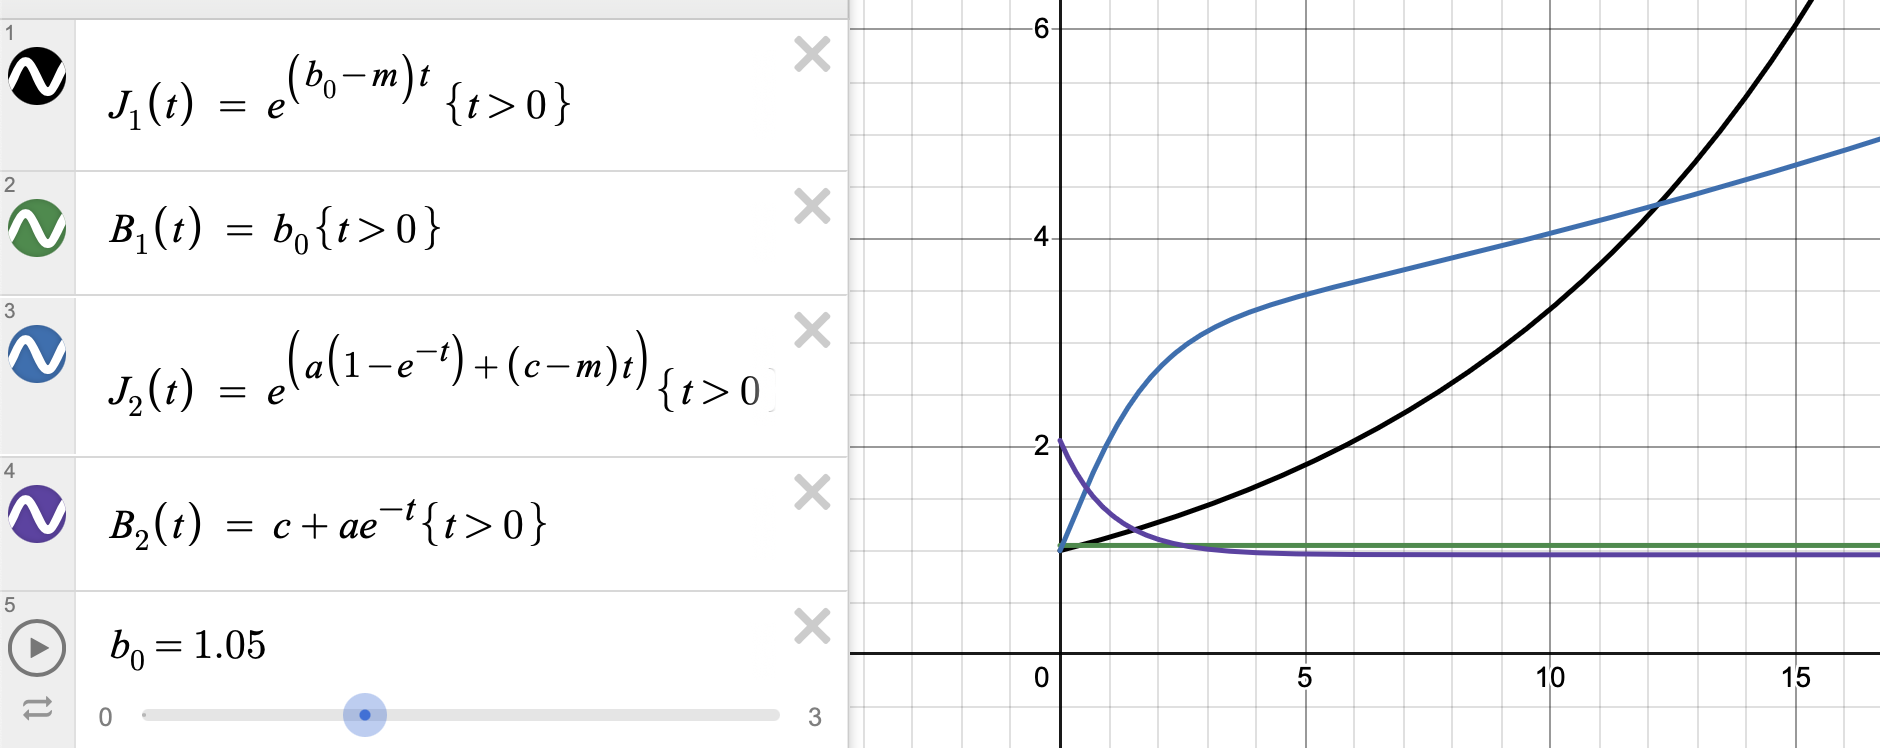
\includegraphics[width=0.99\textwidth]{cmp} % Adjust width as needed
    \caption{Here we see a comparison of the mean (expected values) over time of two branching processes that differ only in birth rate. The black line represents the mean of a simple continuous-time birth-death process in which the death rate is 0.93, and the birth rate is 1.05 (shown with the green line). The comparison case (with mean shown in blue) is also a birth-death process with the same death rate, but with a birth rate that is a decreasing function of time: $\beta = c+a\ee^{-t}$, providing an early replicative boost. The condition of identical replicative potential is imposed by ensuring the area under the birth rate curves is identical between $t=0$ and some time, $t_c$,  seen in the graph at the point where the two means intersect. This remains true regardless of how the parameters are chosen, as long as they meet the stated condition, and this demonstrates that the early advantage does not give an overall advantage.} % Optional caption
    \label{fig:sample-image} % Optional label for referencing
\end{figure}

















































\chapter{ode}




\subsection*{Genetic algorithm for quasistationary formula}
We never found the formula unfortunately, but in principle, I think an approach like this could work.  The code here seeks the correct formula by making a series of itterated modifications in an evolutionary algorithm. Changing both the parameters and the form itself of the equations.  Others have done work like this successfully \cite{cohen2024physics},  and I think ideas from the NEAT algorithm \cite{stanley2002evolving} could crak it if applied successfully. 


\begin{lstlisting}[language=Python]



import numpy as np
import matplotlib.pyplot as plt
from math import floor


'''
The genetic algorithm is used in an attempt to fit a polynomial function to an observed data set.
'''

def read_file(file_path):
    '''Gets the data set from a text file.'''
    X, Y = [], []

    with open(file_path, 'r') as file:
        # Read the entire content as a string
        content = file.read()
        # Alternatively, read the lines of the file into a list
        # lines = file.readlines()
        
        # Process the content as needed

        rows = content.split('\n')
        for row in rows[:-1]:
            items = row.split(',')
            X.append(float(items[0]))
            Y.append(float(items[-1]))
            
    return X, Y


Pvals, Avals = read_file('AdataSave.txt')

# print(Pvals)
# print(Avals)

NumBases = 100 # number of terms in the polynomial
N = 50 # solutions in the evolving population 
mutRate = 0.3 # probability of a given base mutating 

'''The polynomial is of the form sum (a_i P^i). we consider only the first 
NumBases (10) terms. Each cefficient is a rational number of the form a_i = b1_i / b2_i.
A specific polynomial function can hense be described it terms of two lists of 
integers. This is how a particular solution is codefied:
[np.array(b1_1, b1_2, ...), np.array(b2_1, b2_2, ...)].'''


def generateRandomSolution():
    '''Two arrays of 10 integers are generated randomly. Each number is normally 
    distributed with mean 0 and standard deviation, 5.'''
    chrom1 = np.random.normal(0, 5, NumBases).astype(int)
    chrom2 = np.random.normal(0, 5, NumBases).astype(int)
    chrom2 = np.where(chrom2==0, 1, chrom2)
    
    # Fixing the first term to be 1/2 so as to satisfy the IC
    chrom1[0] = 1
    chrom2[0] = 2
    
    trialSolution = [chrom1, chrom2]
    return(trialSolution)

def evaluatePolynomial(P, solution):
    '''Computes the value of a given polynomial for a particular value of P.'''
    polyOut = 0
    for i, tup in enumerate([(n1,n2) for n1,n2 in zip(solution[0], solution[1])]):
        polyOut += (tup[0]/tup[1])*P**i
    return polyOut

def scoreSolution(solution):
    '''Measures the mean squared error between a given polynomial curve and
    the data points.'''
    
    diffs = []
    for i, P in enumerate(Pvals):
        A = Avals[i]
        polyVal = evaluatePolynomial(P, solution)

        squareDiff = (A - polyVal)**2
        diffs.append(squareDiff)
        
    mse = sum(diffs) / len(diffs)
    
    frmZeroSq = evaluatePolynomial(0.5, solution)**2
    
    score = mse + frmZeroSq*100
    
    return(score)



    
    

def plotSolutions(solutionsList):
    '''Takes a list of solutions (polynomials), and plots them all alongside
    the data points. '''
    
    
    # Create the plot
    fig, ax = plt.subplots()
    
    formatPlot(ax)

    ax.scatter(Pvals, Avals, linewidths = 0.2)

    for i, solution in reversed(list(enumerate(solutionsList))):
        
        col = "red" if i == 0 else 'black' 
        alp = 1 if i == 0 else 0.1
        lw = 3 if i == 0 else 1
      
        
        Fvals = []
        X = np.arange(0,0.6,0.01)
        for P in X: 
            Fvals.append(evaluatePolynomial(P, solution))
            
        ax.plot(X, Fvals, color = col, linewidth = lw, alpha = alp)
    
    
    
    
def formatPlot(ax):
    # Add a horizontal line at y=0
    ax.axhline(y=0, color='black', linewidth=0.5)

    # Remove the top and right spines
    ax.spines['top'].set_visible(False)
    ax.spines['right'].set_visible(False)

    # Set the bottom and left spines to be the x and y axis, respectively
    ax.spines['bottom'].set_position(('data', 0))
    ax.spines['left'].set_position(('data', 0))

    # Add a title and axis labels
    ax.set_title("Genetic algorithm converging polynomials")
    ax.set_ylabel("Constant: A(P)", labelpad=5)
    ax.set_xlabel("P")

    # Set the limits of the x and y axes
    ax.set_xlim([0, 0.6])
    ax.set_ylim([0, 0.6])

    # Remove the tick marks on the top and right spines
    ax.xaxis.tick_bottom()
    ax.yaxis.tick_left()

    # Remove the 0.0 tick label from the y-axis
    y_ticks = ax.get_yticks()
    ax.set_yticks([tick for tick in y_ticks if tick != 0])
    

def chooseRandFromOrder(N):
    '''Randomly chooses indecies of a list according to a descending
    geometric distribution.
    This is used to select parents of the next population at random, those 
    with higher fitness being selected with a greater likelihood. '''
    probs = np.array([1/i for i in range(1, N+1)])
    prSum = np.sum(probs)
    probs /= prSum
    
    index = np.random.choice(list(range(N)), p = probs)
    
    return index




def mutate(child):
    '''For a newly generated solution, each number may be moved by + or - 1
    with some mutation probability. If one of the denominators is modified 
    to be 0, the same modification will take place again. For example, if 
    1 is mutated to 0, it will immediately become -1.'''
    for chromIndx in range(2): 
        # The first base location isn't mutated to matain the initial condition
        for baseIndx in range(1, NumBases): 
            if np.random.uniform(0,1) < mutRate:
                #mutation = np.random.choice([-1,1])
                mutation = np.random.normal(0,5,1).astype(int)[0]
                child[chromIndx][baseIndx] += mutation
                if chromIndx == 1 and child[chromIndx][baseIndx] == 0:
                    child[chromIndx][baseIndx] += mutation
                    
    return child

def crossover(parent1, parent2):
    '''Two parent solutions are used to generate one new offspring. Each digit
    of the two lists is taken either from the first parent, or the or the second;
    either option taking place with probabiliy 0.5.'''
    child = [np.zeros(NumBases), np.zeros(NumBases)]

    for chromIndx in range(2): 
        for baseIndx in range(NumBases):
            heritance = None
            
            if np.random.uniform(0,1) < 0.5:
                heritance = parent1[chromIndx][baseIndx]
            else:
                heritance = parent2[chromIndx][baseIndx]
            
            child[chromIndx][baseIndx] = heritance

    return child

def makeNewGeneration(populationSorted): 
    '''A new population is generated by crossing and mutating those of the 
    previous. Fitter solutions are chosen preferentially; the best solution 
    is always kept unchanged, the remaining 49 generated a new.'''
    
    population = [populationSorted[0]] # always keep best
    
    for i in range(N-1): # 49 pairs of parents 
        parent1 = populationSorted[chooseRandFromOrder(N)]
        parent2 = populationSorted[chooseRandFromOrder(N)]
        
        child = crossover(parent1, parent2)
        child = mutate(child)
        
        population.append(child)
    
    return population
    


def sortOnFitness(population, mseVals):
    
    mseIndexTuples = [(mse, i) for i, mse in enumerate(mseVals)]
    mseIndexTuples = sorted(mseIndexTuples)
    
    sortedPopulation = []
    for tup in mseIndexTuples:
        sortedPopulation.append(population[tup[1]])
    
    return sortedPopulation, mseIndexTuples[0][0]







def iterateGeneration(population):
    
    # Score each individual; compute the mean squared error values (fitness)
    mseVals = [scoreSolution(sol) for sol in population]
    
    sortedPopulation, bestMSE = sortOnFitness(population, mseVals)
    print(bestMSE)
    
    plotSolutions(sortedPopulation)#[:10])

    
    newPopulation = makeNewGeneration(sortedPopulation)
    
    return newPopulation

    
# Generate an initial population
population = [generateRandomSolution() for i in range(N)]

numGenerations = 100
for gen in range(numGenerations):
    population = iterateGeneration(population)
    
    
print(population[0])

#1/2 - 1/3 P - 1/6P^2
    
    
    
    

\end{lstlisting}











\subsection*{Logistic speciation code}

Inhomogeneous rate Markov process.  Gillespie algorithm doesn't work -- just discretise time (exact in $\delta t \to 0$ limit.)

\begin{lstlisting}[language=Python]


import numpy as np
from math import log, e
import matplotlib.pyplot as plt



tmax = 15

sims = 10e1

del_t = 0.01


def modSeries(x, y):
    new_x, new_y = [], [y[0]]
    for i in range(len(x)-1):  
        for j in range(2):
            new_x.append(x[i])
            new_y.append(y[i+1]) 
        
    new_x.append(x[-1])
    return(new_x, new_y)


sig = 2
K = 4
n0 = 2
xi = K/n0 -1
r = 0.8

def N(t):
    return K*e**(r*t) / (xi + e**(r*t))

def b2(t):
    return sig * r * N(t) * (1 - N(t)/K)

def beta(t):
    return sig * K * (xi / (xi + e**(r*t)))

mu = 0.4



def run_episode():

    
    t = 0
    X = 1
    
    time_series = np.array([[0, X]])
    
    itr = 0

    while t+del_t < tmax and itr < 100000:
        itr += 1
        
        U = np.random.uniform(0,1)
        
        birth_prob = b2(t) * X * del_t
        death_prob = mu * (X-1) * del_t
        
        if U < birth_prob: 
            X += 1
        elif U < birth_prob + death_prob: 
            X -= 1
        else:
            pass 
   
        t += del_t
        
        time_series = np.append(
            time_series,
            [[t,X]], axis=0
            )
        
  
        
    return(time_series)
        






def get_data():
    
    data = []
    
    for i in range(int(sims)): 
        data.append(run_episode()) 
    
    return(data) 

data = get_data()


# Change to use the newly defined alpha value 

def calc_averages(data): 
    
    # maxTime = tmax
    
    # alpha = del_t

    # calculates rolling time series averages for M, E and I
    # size of uniform time step
    
    # sets up uniform time steps for plotting the x axis
    timeSteps = data[0][:,0]
    
   
    # # time series for the average of macrophages
    X_avg = np.zeros(timeSteps.size)

    for timeSeries in data:
        
        for i, step in enumerate(timeSeries): 
            
            X_avg[i] += step[1]
    
    X_avg /= sims

    
    
    return(timeSteps, X_avg)




\end{lstlisting}













\subsection*{Allogorical model code (vitality birth death catastrophe)}

Inhomogeneous Markov process coupled with an ODE,  each discretised in time.  ODE solved with Euler method.  

\begin{lstlisting}[language=Python]


import numpy as np
from math import log, e
import matplotlib.pyplot as plt




def euler(var, X, t, f, dt):
    return var + f(var, X, t)*dt




##################################################### Gillespie 

def modSeries(x, y):
    new_x, new_y = [], [y[0]]
    for i in range(len(x)-1):  
        for j in range(2):
            new_x.append(x[i])
            new_y.append(y[i+1]) 
        
    new_x.append(x[-1])
    return(new_x, new_y)



def N(t):
    return K*e**(r*t) / (xi + e**(r*t))

def b2(t):
    return sig * r * N(t) * (1 - N(t)/K)

def beta(t):
    return sig * K * (xi / (xi + e**(r*t)))






tmax = 30

sims = 10e1

del_t = 0.001




sig = 2
K = 4
n0 = 2
xi = K/n0 -1
r = 0.8


mu = 0.4


xi = 2
eta = 0.001

# single ODE describing the behaviour of S0
def N_ODE(N, X, t):
    
    dNdt = xi - eta * X * N
    
    return dNdt



def run_episode():

    
    t = 0
    X = 1
    N = 1 # change
    
    t_series = np.array([0])
    X_series = np.array([X])
    N_series = np.array([N])
    
    itr = 0

    while t+del_t < tmax and itr < 100000:
        itr += 1
        
        U = np.random.uniform(0,1)
        
        
        
        birth_prob = 0.1 * N  * X * del_t
        death_prob = 0.06 * X * del_t
        
        cat_prob = (0.0001/N) * X * del_t
        
        
        
        
        #N = euler(N, t, N_ODE, del_t)
        
        if X > 0:
            
            if U < birth_prob: 
                X += 1
            elif U < birth_prob + death_prob: 
                X -= 1
            elif U < birth_prob + death_prob + cat_prob:
                X = 0
            else:
                pass 
            
        else:
            
            inj_rate = 0.1
            if U < inj_rate:
                X = 1
            
        
        N = euler(N, X, t, N_ODE, del_t)
        
        
   
        t += del_t
        
        t_series = np.append( t_series, [t], axis=0)
        X_series = np.append( X_series, [X], axis=0)
        N_series = np.append( N_series, [N], axis=0)
        
  
        
    return(t_series, X_series, N_series*100)
        


# Loop to plot multiple episodes
for i in range(1):
    ts, xs, ns = run_episode()
    plt.plot(ts, xs, color="blue")   # No label here to avoid duplicate entries in the legend
    plt.plot(ts, ns, color="orange") # No label here either

# Add labels and legend once, outside the loop
plt.xlabel("time $t$")
plt.plot([], [], label="$X_t$", color="blue")   # Adding empty plots with labels for legend
plt.plot([], [], label="$N(t)$", color="orange")
plt.legend()

\end{lstlisting}




\subsection*{Birth plague model code}


\begin{lstlisting}


import numpy as np
from math import log

import matplotlib.pyplot as plt

lamb = 1
gama = 0.1
beta = 0.02 
mu = 10


X = 1
Y = 0


data = []

baseRates = np.array([lamb, gama, beta, mu])  # birth corruption infection death`

activeRates = np.array([])


def update_active_rates():
    global activeRates
    rateMultipliers = np.array([X, X, X*Y, Y])
    activeRates = baseRates * rateMultipliers
    
update_active_rates()
  

print(np.sum(activeRates))


t = 0
step = 0

maxTime = 20
maxSteps = 10e4


dataX = [X]
dataY = [Y]
dataT = [0]


def event_birth():
    global X
    X += 1
    
def event_deathY():
    global Y
    Y -= 1

def event_corruption():
    global X, Y 
    X -= 1
    Y += 1
    
def event_infection():
    global X, Y
    X -= 1
    Y +=1

eventProbs = activeRates / np.sum(activeRates)

print(activeRates)
print(eventProbs)

eventIndex = np.random.choice([0, 1, 2, 3], p=eventProbs) 

update_active_rates()


while t < maxTime and step < maxSteps and X+Y>0:
    
    update_active_rates()
    rateSum = np.sum(activeRates)
    eventProbs = activeRates / rateSum
    
    U = np.random.uniform(0, 1)
    
    # get time to next event 
     
     # generate uniform random, U
     # inter event time = -log(U)/RateSum
     
    timeStep = -log(U)/rateSum
    t += timeStep
    
    ev_In = np.random.choice([0,1,2,3], p=eventProbs) # event index 
    # birth corruption infection death`
    
    print(ev_In)
    
    if (ev_In == 0):
        # birth
        event_birth()
    elif (ev_In == 1):
        # corruption 
        event_corruption()
    elif (ev_In == 2): 
        # infection 
        event_infection()
    elif (ev_In == 3):
        # death 
        event_deathY()
        
        
    print(X, Y)
    
    
    dataX.append(X)
    dataY.append(Y)
    dataT.append(t)
    

    step += 1
   
    

\end{lstlisting}

